\documentclass{article}
\usepackage{graphicx} % Required for inserting images
\usepackage[top=0.9in, bottom=1in, left=1.5in, right=1.5in]{geometry}
\usepackage[utf8]{inputenc}
\usepackage[icelandic]{babel}
\usepackage[T1]{fontenc}
\usepackage[sc]{mathpazo}
\usepackage[parfill]{parskip}
\renewcommand{\baselinestretch}{1.2}
\usepackage{booktabs,tabularx}
\usepackage{multirow}
\usepackage{enumerate}
\usepackage{adjustbox}
\usepackage{multicol}
\usepackage{xcolor}
\usepackage{algpseudocode}
\usepackage{tikz}
\usepackage{nicefrac}
\usepackage{changepage}
\usetikzlibrary{arrows, positioning, calc, graphs}
\usepackage{amsmath, amsfonts, amssymb, amsthm}
\usepackage{graphicx}
\usepackage{tikz}
\usepackage{minted}
\usemintedstyle{manni}
\title{Forritunarmál Einstaklingsverkefni 9}
\author{Ragnar Björn Ingvarsson, rbi3}
\tikzset{->, >=stealth', shorten >=1pt, node distance=2cm,thick, main node/.style={circle,draw,minimum size=3em}}

\begin{document}
\renewcommand\thepage{}

	\maketitle

	\newpage
	\begin{verbatim}
{;;;

Design document for "complex.mmod"
==================================

Exported
--------

Use:  z = complex(x,y);
Pre:  x and y are floating point numbers.
Post: z is the complex number x+yi.

Use:  x = real(z);
Pre:  z is a complex number.
Post: x is the real part of z.

Use:  x = imag(z);
Pre:  z is a complex number.
Post: x is the imaginary part of z.

Use:  z = x+++y;
Pre:  x and y are complex numbers.
Post: z is a complex number that is the sum of x and y.

Use:  z = x---y;
Pre:  x and y are complex numbers.
Post: z is a complex number that is the difference of x and y.

Use:  z = x***y;
Pre:  x and y are complex numbers.
Post: z is a complex number that is the product of x and y.

Use:  z = x///y;
Pre:  x and y are complex numbers.
      y is not zero.
Post: z is a complex number that is the quotient of x and y.

Imported
--------

Only BASIS function are imported.

;;;}

"complex.mmod" =
!{{
;;; Data invariant:
;;;   A complex number z = x+yi, where x and y
;;;   are double numbers, is represented as the pair [x$y].

+++ =
    fun(x,y)
    {
        return complex(real(x) + real(y), imag(x) + imag(y));
    };
    
--- =
    fun(x,y)
    {
        return complex(real(x) - real(y), imag(x) - imag(y));
    };

*** =
    fun(x,y)
    {
        var xr = real(x);
        var xi = imag(x);
        var yr = real(y);
        var yi = imag(y);
        return complex(xr * yr - xi * yi, xr * yi + xi * yr);
    };


/// =
    fun(x,y)
    {
        var xr = real(x);
        var xi = imag(x);
        var yr = real(y);
        var yi = imag(y);
        val d = yr * yr + yi * yi;
        return complex((xr * yr + xi * yi)/d, (xi * yr - xr * yi)/d);
    };

complex =
    fun(x,y)
    {
        return [x$y];
    };

real =
    fun(z)
    {
        return head(z);
    };

imag =
    fun(z)
    {
        return tail(z);
    };
}}
;

	\end{verbatim}
	\begin{center}
		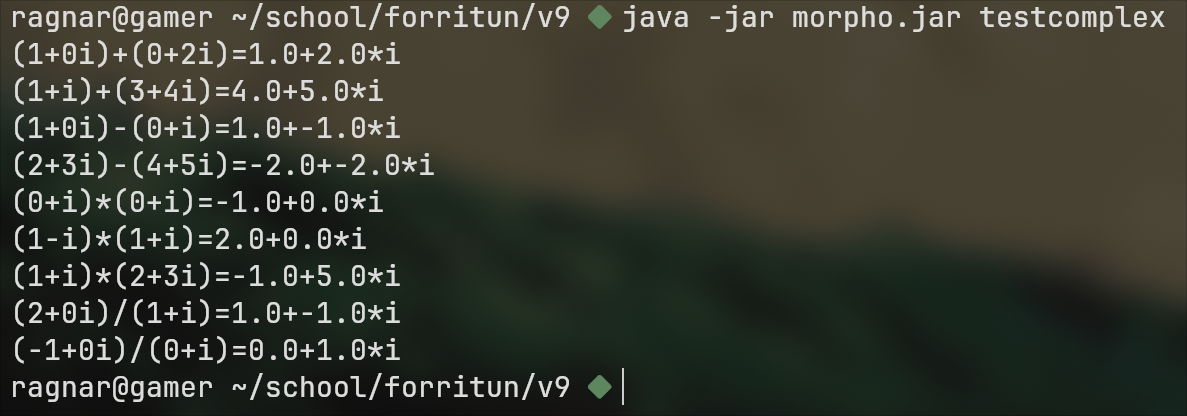
\includegraphics[scale=0.33]{complex.png}
	\end{center}
	
\end{document}
